\documentclass{article}

% - style template
\usepackage{base}

% - title, author, etc.
\title{COMP3007 - Assignment}
\author{Tom Ross}
\date{\today}

% - headers
\pagestyle{fancy}
\fancyhf{}
\rhead{\theauthor}
\chead{}
\lhead{\thetitle}
\rfoot{\thepage}
\cfoot{}
\lfoot{}

% - document
\begin{document}

The entire code repository can be found at
\url{https://github.com/dgsaf/comp3007_assignment}.

\tableofcontents

\listoffigures

\listoftables

\clearpage

\section{Introduction}
\label{sec:introduction}

\section{Problem Analysis}
\label{sec:problem-analysis}

We are concerned with the detection and classification of two similar but
distinct types of signs.
The properties specific to each type of signage are discussed in
\autoref{sec:problem-1} and \autoref{sec:problem-2}.
Here, we remark on the properties common to both of them, which are numerous and
allow for a broadly unified approach to their detection and classification.

Each sign consists of a black background with white characters (digits and
directional arrows) forming the foreground of the sign.
The black background is rectangular in shape, and bounds the characters
regions.
Furthermore, the contrast between the black background and the white foreground
is strong across all colour channels and in grayscale.

The digits are uniform in their construction, being printed in a monospace
font with fixed height and allocated a fixed width; although each digit does
not necessarily fully extend across its allocated width - as can be seen for the
digit 1.
Likewise, the directional arrows are also uniform in their construction but
their dimensions are distinct from those of the digits - noticeably having a
smaller height than the digits.

The digits do not overlap with each other (unless subject to camera
artifacts/blurring) but are closely adjacent to each other, and regularly
spaced.
Each sign contains at least one sequence of three digits, which are ideally
surrounded by a black sub-region of the sign; although for task 2, the gap
between the leftmost digit and the edge of the sign can be very small.

In summary, the following properties of the signs are almost always observed,
providing a robust foundation for their detection:
\begin{itemize}
\item
  The uniformly white colour of the characters;

\item
  The uniformly black background of the sign;

\item
  The strong contrast between the white characters and the black background
  across all red, green, and blue channels as well as in grayscale;

\item
  The uniform height of the digits;

\item
  The uniform spacing of the characters horizontally;

\item
  The height of the digits exceeding the width;

\item
  The uniform dimensions of the arrows;

\item
  The presence of a chain of exactly three digits;

\item
  A sizeable sub-region of the sign above and below the chain of digits, which
  is uniformly black.
\end{itemize}
However, the assumption of the above properties may be invalidated by any one of
the (non-exhaustive) list of conditions:
\begin{itemize}
\item
  The presence of strong radial, or motion blurring which may cause character to
  overlap;

\item
  The presence of strong shadowns, glare, or other variations in lighting
  conditions across the character;

\item
  The presence of a foreign object, such as a sticker or a mark, on the sign
  (violating the assumptions on uniformity of layout) or across the characters
  (violating the assumptions on uniformity of characters).

\end{itemize}
It should also be noted that often there are other monospace white characters
present near the sign - typically letters forming the name of the location
marked by the sign.
These characters can be distinguished from the digits (and arrows) by the fact
that they almost always form chains of more than three characters, and presented
on their own signs which almost never have a black background.

\subsection{Task 1}
\label{sec:problem-1}

Further refinement of the problem analysis is possible for task 1.
We are concerned with finding only one chain of three digits, and we are not
concerned with directional arrows at all.
Futhermore, there exists a sizeable gap between the chain of digits and the edge
of the sign both horizontally and vertically.

Bricks and other objects which are of approximately uniform dimensions and
uniformly spaced are regularly present in images for task 1 - hence, when
exploiting the uniformity of the layout of the digits, care must be taken to
avoid or handle the false detection of these other objects.

Examples of the images expected for task 1, which provide the justification for
the assumptions made on the properties of the sign are shown in
\autoref{fig:problem-1-regular}.
Examples of images which may be encountered for task 1, but which challenge the
assumptions made on the properties of the sign are shown in
\autoref{fig:problem-1-outlier}.

\begin{figure}[h]
  \centering
  \begin{subfigure}[t]{0.22\textwidth}
    \centering
    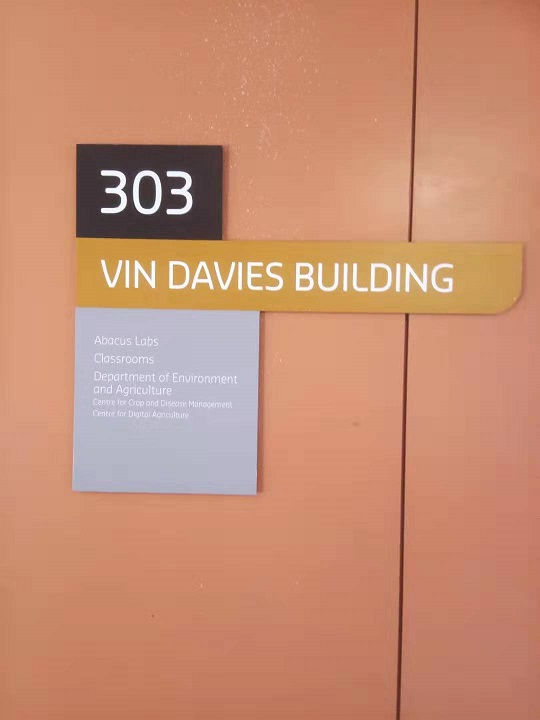
\includegraphics[width=0.9\textwidth]{../train/task1/BS02}
    \caption[BS02]{
      \lstinline{BS02.jpg}
    }
    \label{fig:bs02}
  \end{subfigure}
  %
  \begin{subfigure}[t]{0.22\textwidth}
    \centering
    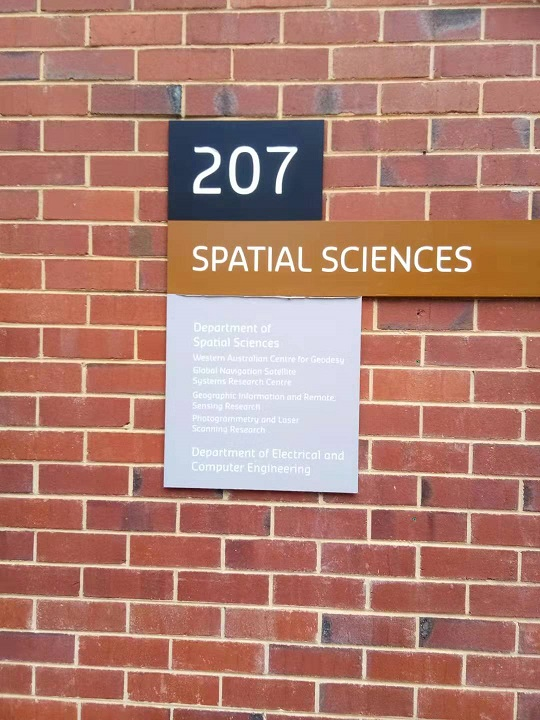
\includegraphics[width=0.9\textwidth]{../train/task1/BS04}
    \caption[BS04]{
      \lstinline{BS04.jpg}
    }
    \label{fig:bs04}
  \end{subfigure}
  %
  \begin{subfigure}[t]{0.22\textwidth}
    \centering
    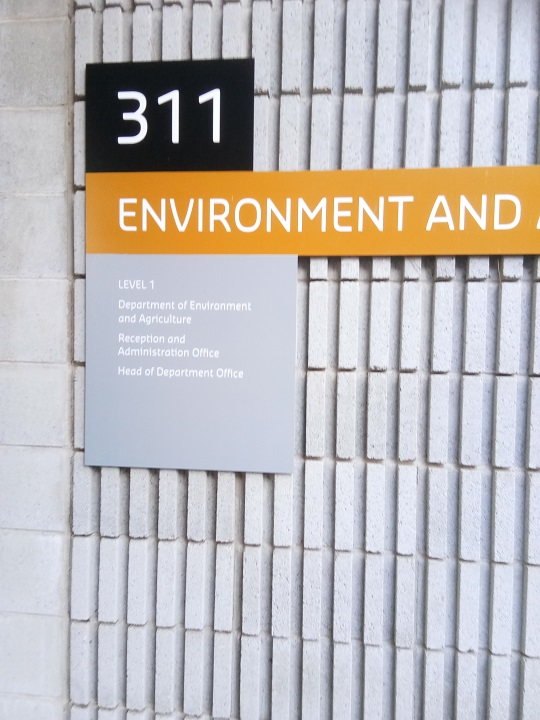
\includegraphics[width=0.9\textwidth]{../train/task1/BS09}
    \caption[BS09]{
      \lstinline{BS09.jpg}
    }
    \label{fig:bs09}
  \end{subfigure}
  %
  \begin{subfigure}[t]{0.22\textwidth}
    \centering
    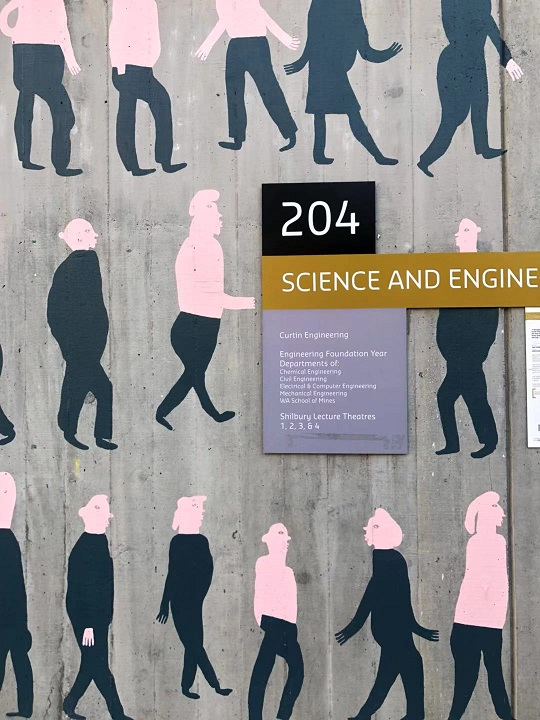
\includegraphics[width=0.9\textwidth]{../train/task1/BS14}
    \caption[BS14]{
      \lstinline{BS14.jpg}
    }
    \label{fig:bs14}
  \end{subfigure}

  \caption[Task 1 - Regular Cases]{
    Examples of training images for task 1, which exhibit the described
    distinguishing properties of the signs and digits.
  }
  \label{fig:problem-1-regular}
\end{figure}

\begin{figure}[h]
  \centering
  \begin{subfigure}[t]{0.22\textwidth}
    \centering
    
\includegraphics[width=0.9\textwidth]{../train/task1/BS03}
    \caption[BS03]{
      \lstinline{BS03.jpg}
    }
    \label{fig:bs03}
  \end{subfigure}
  %
  \begin{subfigure}[t]{0.22\textwidth}
    \centering
    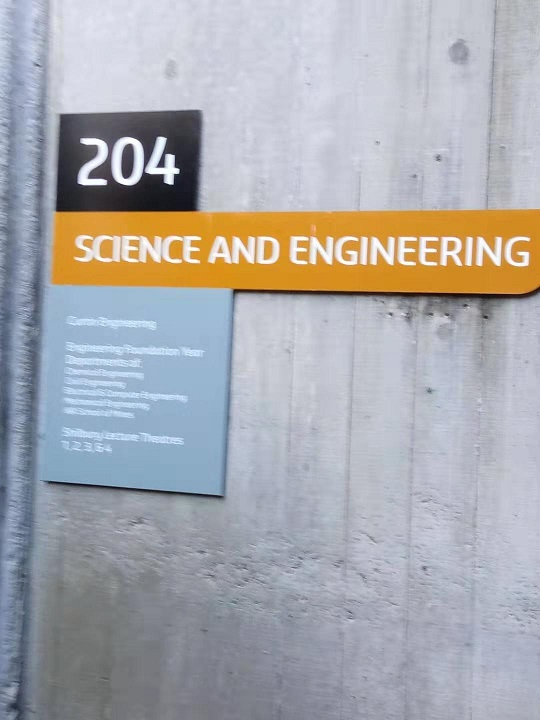
\includegraphics[width=0.9\textwidth]{../train/task1/BS05}
    \caption[BS05]{
      \lstinline{BS05.jpg}
    }
    \label{fig:bs05}
  \end{subfigure}
  %
  \begin{subfigure}[t]{0.22\textwidth}
    \centering
    
\includegraphics[width=0.9\textwidth]{../train/task1/BS07}
    \caption[BS07]{
      \lstinline{BS07.jpg}
    }
    \label{fig:bs07}
  \end{subfigure}
  %
  \begin{subfigure}[t]{0.22\textwidth}
    \centering
    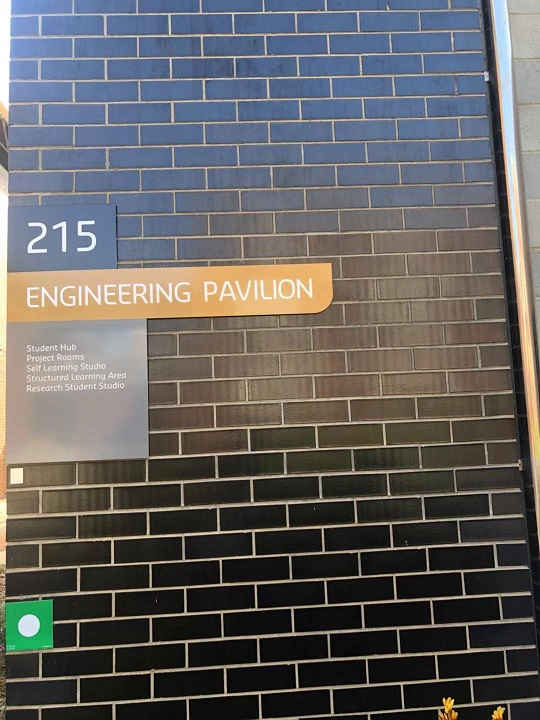
\includegraphics[width=0.9\textwidth]{../train/task1/BS11}
    \caption[BS11]{
      \lstinline{BS11.jpg}
    }
    \label{fig:bs11}
  \end{subfigure}

  \caption[Task 1 - Edge Cases]{
    Examples of training images for task 1, which may challenge the assumptions
    made on the signs and thus necessitate the development of a robust detection
    algorithm.
    Sharp shadows, motion blur and monochromatic periodic objects, which may
    interfere with digit detection, can be observed.
  }
  \label{fig:problem-1-outlier}
\end{figure}

\subsection{Task 2}
\label{sec:problem-2}

Similarly, further refinement of the problem analysis is possible for task 2.
We are concerned with finding a variable number of chains of three digits, each
of which has an associated directional arrow to their right.
For each chain and their associated directional arrow, the geometric centres of
the digits are arrow are collinear; hence we say that they form a line.
Each line is vertically spaced (by a distance just larger than the height of the
digits) and the set of digits and arrows from each line thus forms a grid-like
layout.

A challenging aspect of these signs, compared to those for task 1, is that the
gap between the leftmost digit on each line and the edge of the sign can be very
small.
In cases where an object, of similar colour/intensity to the white characters,
is behind the sign but in a similar region of the image to the leftmost digit of
a line, the digit and the object may prove difficult to distinguish as separate
regions.

Another difficulty is that the number of lines in any particular sign is not
known beforehand.
However, there is a benefit in having multiple lines per sign as it provides a
mechanism, given at least one fully known line or even partial information from
multiple lines, to recover an expected location for characters which fail to be
detected initially.

Similar to task 1, the scene environment can be expected to be quite noisy, with
periodically repeating objects such as brickwork present, as well as other
objects with many sharp edges, such as plants and trees.
It also seen that foreign objects, such as stickers and marks, may be present on
the signs, and that other objects, such as plants, may occlude the sign itself.

Examples of the images expected for task 2, which provide the justification for
the assumptions made on the properties of the sign are shown in
\autoref{fig:problem-2-regular}.
Examples of images which may be encountered for task 2, but which challenge the
assumptions made on the properties of the sign are shown in
\autoref{fig:problem-2-outlier}.

\begin{figure}[h]
  \centering
  \begin{subfigure}[t]{0.22\textwidth}
    \centering
    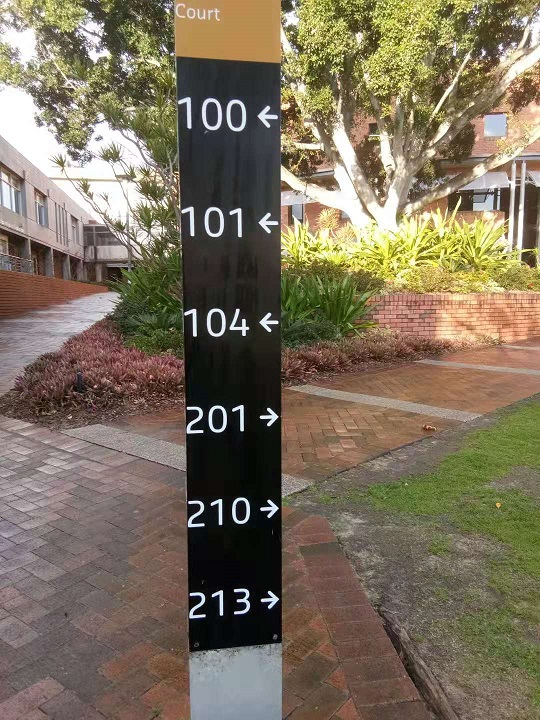
\includegraphics[width=0.9\textwidth]{../train/task2/DS06}
    \caption[DS06]{
      \lstinline{DS06.jpg}
    }
    \label{fig:ds06}
  \end{subfigure}
  %
  \begin{subfigure}[t]{0.22\textwidth}
    \centering
    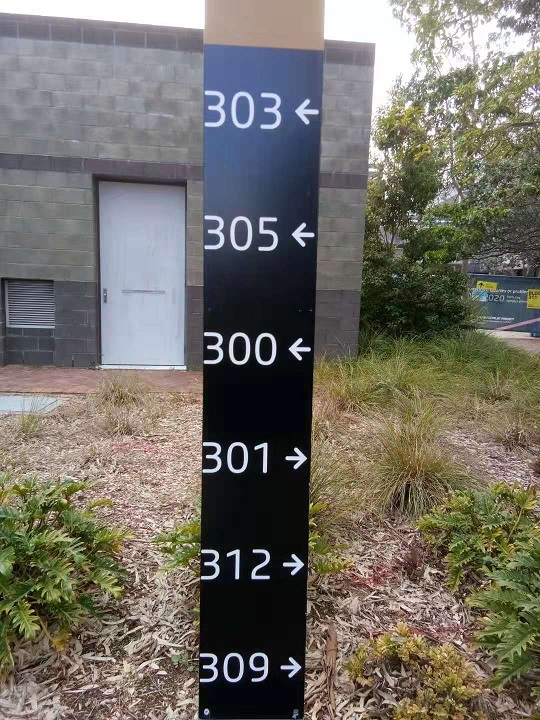
\includegraphics[width=0.9\textwidth]{../train/task2/DS12}
    \caption[DS12]{
      \lstinline{DS12.jpg}
    }
    \label{fig:ds12}
  \end{subfigure}
  %
  \begin{subfigure}[t]{0.22\textwidth}
    \centering
    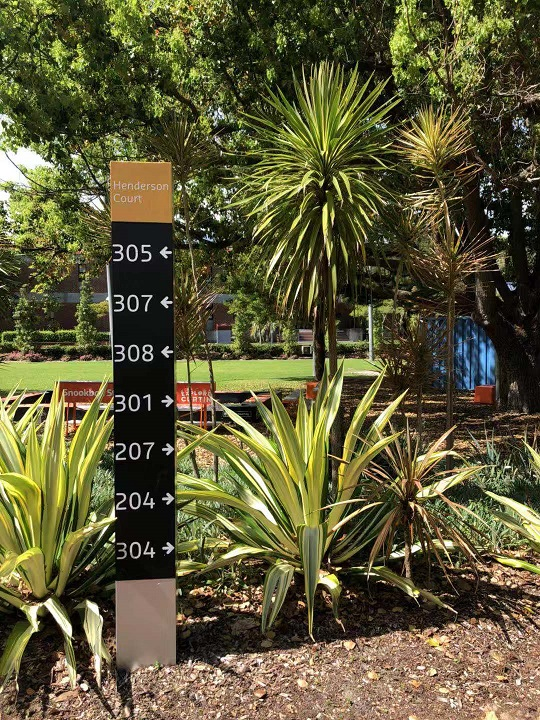
\includegraphics[width=0.9\textwidth]{../train/task2/DS13}
    \caption[DS13]{
      \lstinline{DS13.jpg}
    }
    \label{fig:ds13}
  \end{subfigure}
  %
  \begin{subfigure}[t]{0.22\textwidth}
    \centering
    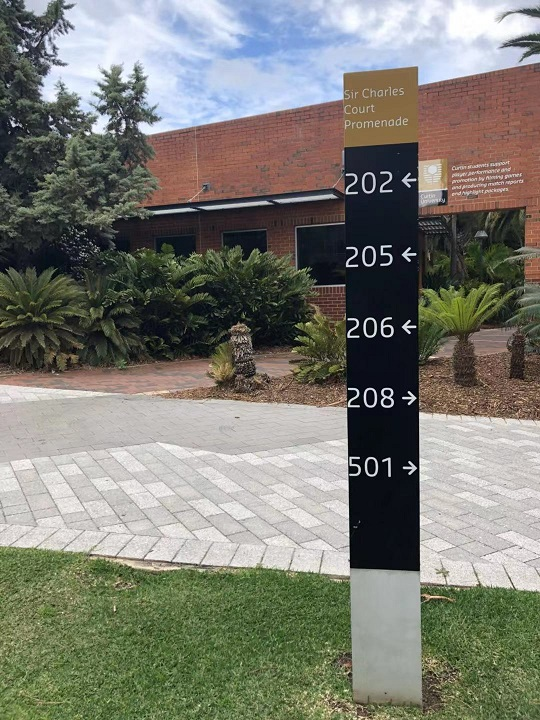
\includegraphics[width=0.9\textwidth]{../train/task2/DS18}
    \caption[DS18]{
      \lstinline{DS18.jpg}
    }
    \label{fig:ds18}
  \end{subfigure}

  \caption[Task 2 - Regular Cases]{
    Examples of training images for task 2, which exhibit the described
    distinguishing properties of the signs, and their digits and arrows.
  }
  \label{fig:problem-2-regular}
\end{figure}

\begin{figure}[h]
  \centering
  \begin{subfigure}[t]{0.22\textwidth}
    \centering
    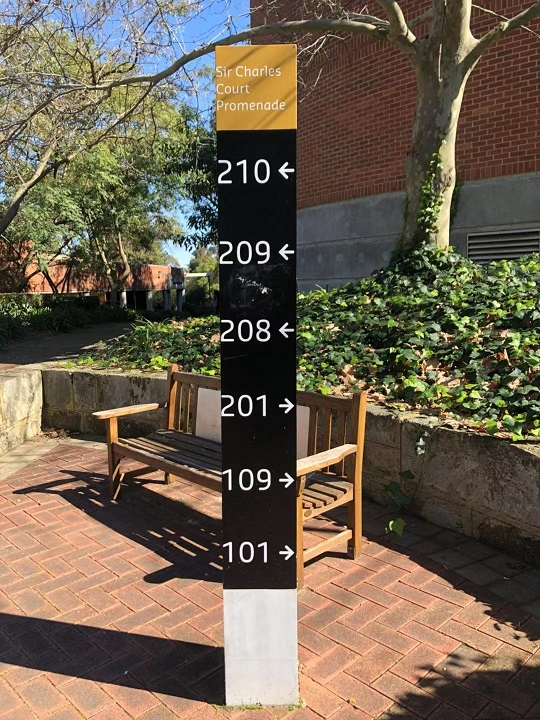
\includegraphics[width=0.9\textwidth]{../train/task2/DS02}
    \caption[DS02]{
      \lstinline{DS02.jpg}
    }
    \label{fig:ds02}
  \end{subfigure}
  %
  \begin{subfigure}[t]{0.22\textwidth}
    \centering
    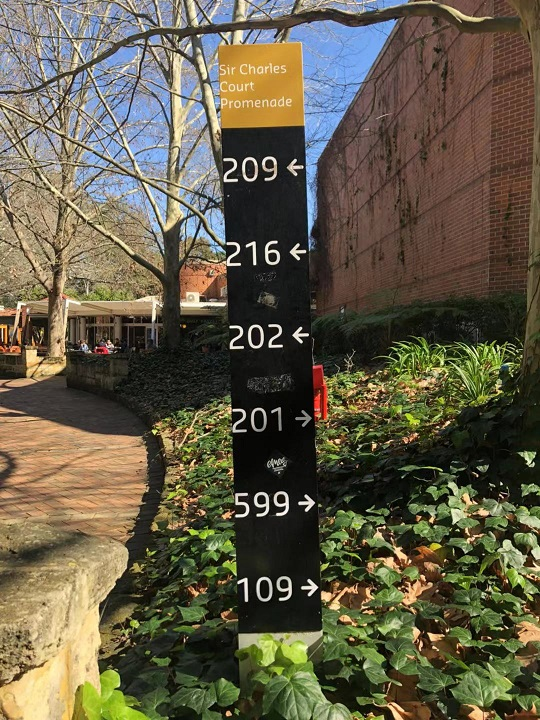
\includegraphics[width=0.9\textwidth]{../train/task2/DS07}
    \caption[DS07]{
      \lstinline{DS07.jpg}
    }
    \label{fig:ds07}
  \end{subfigure}
  %
  \begin{subfigure}[t]{0.22\textwidth}
    \centering
    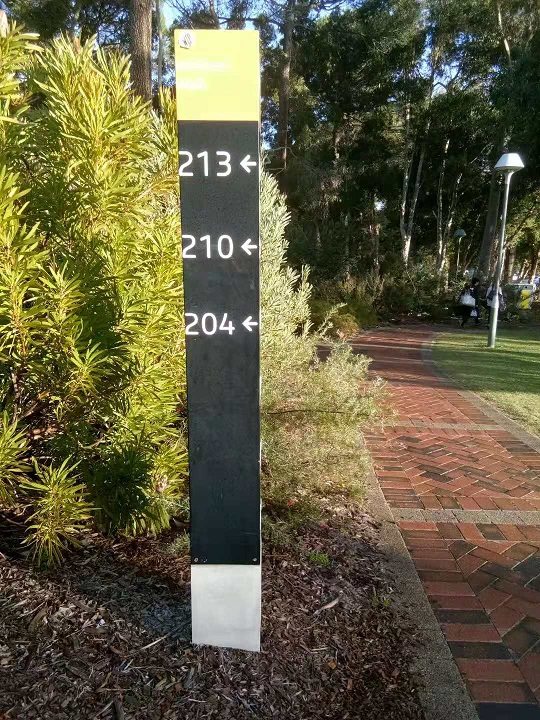
\includegraphics[width=0.9\textwidth]{../train/task2/DS10}
    \caption[DS10]{
      \lstinline{DS10.jpg}
    }
    \label{fig:ds10}
  \end{subfigure}
  %
  \begin{subfigure}[t]{0.22\textwidth}
    \centering
    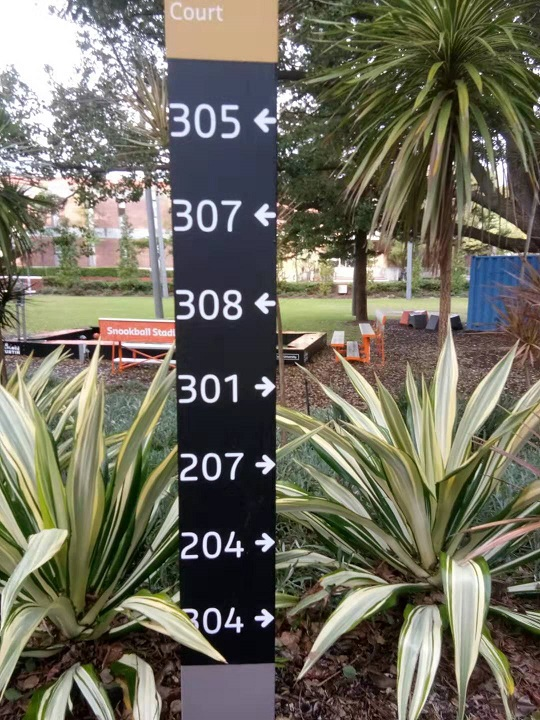
\includegraphics[width=0.9\textwidth]{../train/task2/DS11}
    \caption[DS11]{
      \lstinline{DS11.jpg}
    }
    \label{fig:ds11}
  \end{subfigure}

  \caption[Task 2 - Edge Cases]{
    Examples of training images for task 2, which may challenge the assumptions
    made on the signs and thus necessitate the development of a robust detection
    algorithm.
    Characters overlapping with similar regions outside the sign, foreign
    objects on the sign, variable lighting conditions can all be observed.
  }
  \label{fig:problem-2-outlier}
\end{figure}

\clearpage

\section{Implementation}
\label{sec:imp}

\subsection{Overview}
\label{sec:imp-overview}

We make use of the commonality of the properties of the signs that are to be
detected in task 1 and task 2 by designing a detection algorithm which can be
adapted with minor changes for each task.
The specific detection algorithms for each task are discussed in
\autoref{sec:imp-1} and \autoref{sec:imp-2}.
Furthermore, as the digits to be classified in each task are of the same style,
we also design a classification algorithm which is suitable for both tasks.
Naturally, a separate classifier will be needed for the directional arrows,
however we use the $k$-Nearest Neighbours ($k$-NN) algorithm for classifying
both the digits and the arrows.
Hence, we discuss the problem of classification, for both types of characters,
in a general manner in \autoref{sec:imp-classification}.

\subsection{Detection}
\label{sec:imp-detection}

To detect the characters (digits and arrows) we utilise the method of
Maximally Stable Extremal Regions (MSER) - first developed by
\cite{MATAS2004761}.
We present our formalism in a similar manner to \cite{MATAS2004761}.
In this method, a number of regions, which are extremal in terms of light
intensity and stable in the sense that the region boundary changes little under
a varying threshold, are detected in the grayscale image.
We suggest that this technique is suitable for our purpose, as the characters
are uniformly white and contrast well against the surrounding uniformly black
bounding area of the signs.
Furthermore, in most cases the characters are well separated from other
characters and the edge of the sign (except notably for the leftmost digits in
task 2).
Hence, these characters should form extremal regions which are relatively stable
under affine transformations, and when the image is underexposed or overexposed.
Theoretically, this technique may be susceptible to extreme variations in
lighting conditions, such as strong shadows or glare, which form discontinuous
non-monotonic changes in light intensity.
However, in testing, this technique has proved tolerant to moderate shadows and
glare, so we do not expect this to be a major issue.

With suitably chosen parameters for the MSER algorithm, the regions of interest,
corresponding to the characters on the sign, can be reliably detected - but must
be distinguished from the other regions detected which are not of interest.
Using known properties of the characters (such as dimension, aspect ratio,
bounding box fill) we are able to refine the set of regions.

To detect the regions corresponding to the sequences of digits, we then examine
the geometric relationships between the regions to determine which pairs of
regions are: similar in dimension, and possibly collinear.
This results in a directed graph of regions, with paths in this graph
constituting possible lines of similar regions.
For each region in this graph we filter their set of edges to leave only the
edge connecting it to the closest adjacent region - ensuring all paths are
non-overlapping.
We then extract all possible paths, which we call chains, and analyse each chain
by length and by contrast (in gray scale as well as in red, green, and blue
channels) to order the chains by their likelihood of being a sequence of three
digits.

For task 1, we detect only the most likely chain as our sequence of digits, and
the problem of detection is complete.
For task 2, we cluster these chains by their likelihood and select the most
likely subset of the chains.
If any of the sequences of digits have been only partially found (e.g. two out
of three digits), we make use of the grid-like layout of the digits to locate
the remaining digit.
A bounding box is drawn around where the remaining digit is expected to be
present, and a connected-components algorithm is employed to construct a region
for this digit which is limited to the scope of this bounding box.
With all regions corresponding to the digit sequences now found, the
collinearity of the digits is used to locate the region corresponding to the
directional arrow associated with these digits.
Thus for each task, the detected lines of digits (and directional arrows for
task 2) are now located.

\subsection{Classification by $k$-Nearest Neighbours}
\label{sec:imp-classification}

Prior to the classification stage, we note that we could use the collinearity of
the lines, and the uniform height of the digits, to construct an affine, or even
a perspective, transformation which rotates the line to be horizontal.
However, it was observed in training and validation that the detection and
classification algorithms performed well enough with out the need for a
perspective transformation.

To address the problem of digit and directional arrow classification, we use
the $k$-NN algorithm, comparing the regions expected to be digits and arrows
with the training digits and arrows respectively.
For each region, we define a binary image (with the dimensions of the bounding
box of the region) which maps each point that is in the region to 1, and 0
otherwise.
We then decompose the binary image into a set of bins (which are symmetric about
the bounding box midpoint) and use the spatial occupancy of each bin as a
feature vector for the region.
We suggest that this approach is suitable, as the digits and directional arrows
are of a uniform style and dimensions, and we note that this feature vector is
scale-invariant.
In testing with a suitably selected number of bins, this approach has proved to
be reliably accurate despite its simplicity.

\subsection{Mathematical Details}
\label{sec:mathematical-details}

We introduce here various formal presentations of the concepts used in the
detection and classification algorithms.

\subsubsection*{Image}

We define an image $I$, with $n$ channels and of width $w$ and height $h$, to be
a mapping
\begin{equation}
  \label{eq:def-image}
  I
  :
  D \to S
  :
  \lr{x, y}
  \mapsto
  I\lr{x, y}
  =
  \lr[\big]
  {
    I_{1}\lr{x, y}
    ,
    \dotsc
    ,
    I_{n}\lr{x, y}
  }
  ,
\end{equation}
where the domain $D \subset \natural^{2}$ is of the form
$D = \lrset{0, \dotsc, w - 1} \times \lrset{0, \dotsc, h - 1}$, and $S$ is the
codomain.
Constraints can be specified on $S$, but for our purposes it suffices to suppose
that either $S \subseteq \lrset{0, \dotsc, 255}^{n}$ or $S \subset \real^{n}$.

\subsubsection*{Thresholded Image}

Suppose $I : D \to S \subset \real$ is a single-channel image.
For each $t \in S$, we define the Boolean-valued image $I_{t}$ to be of the
form
\begin{equation}
  \label{eq:def-image-threshold}
  I_{t}
  :
  D \to \mathbb{B}
  :
  \lr{x, y}
  \mapsto
  \begin{cases}
    0
    &\qq{if}
    I\lr{x, y} \leq t
    \\
    1
    &\qq{if}
    I\lr{x, y} > t
  \end{cases}
  ,
\end{equation}
and we say that $I_{t}$ is a thresholded image.

\subsubsection*{Otsu Separation}

Suppose that $I : D \to S \subset \real$ is a single channel image.
Let $t \in S$ be the threshold which maximises the inter-class variance of
the binary distribution $I_{t}\lr{D}$, which is obtained via Otsu's method.
The mean of each class $k \in \lrset{0, 1}$ is of the form
\begin{equation}
  \label{eq:def-otsu-mean}
  \mu_{k}\lr{I}
  =
  \sum_{p \in D : I_{t}\lr{p} = k}
  I\lr{p}
  .
\end{equation}
We define the Otsu separation $\varsigma\lr{I}$ of $I$ to be the difference of
these means; that is,
\begin{equation}
  \label{eq:def-otsu-separation}
  \varsigma\lr{I}
  =
  \mu_{1}\lr{I}
  -
  \mu_{0}\lr{I}
  .
\end{equation}

\subsubsection*{Bounding Box}

Suppose $D$ is the domain of an image $I : D \to S$.
For all $R \subseteq D$, we define the bounding box $B\lr{R}$ of $R$ to be
\begin{equation}
  \label{eq:def-bounding-box}
  B\lr{R}
  =
  \lrsq{x_{R}, x_{R} + w_{R}}
  \times
  \lrsq{y_{R}, y_{R} + h_{R}}
  \qq{such that}
  R \subseteq B\lr{R}
\end{equation}
and where $w_{R}, h_{R} \in \natural$ are minimal.

\subsubsection*{Connectedness}

Suppose $D$ is the domain of an image.
An adjacency relation $A$ on $D$ is a Boolean-valued mapping
\begin{equation}
  \label{eq:def-adjacency}
  A
  :
  D \times D \to \mathbb{B}
  :
  \lr{p, q}
  \mapsto
  A\lr{p, q}
  ,
\end{equation}
which indicates if the two points of the domain are considered to be adjacent.
For any $p \in D$, we may define the neighbourhood $N\lr{p}$ of $p$ to be the
set of all points which are adjacent to it; that is,
\begin{equation}
  \label{eq:def-neighbourhood}
  N\lr{p}
  =
  \lrset
  {
    q \in D
    \mid
    A\lr{p, q}
  }
  .
\end{equation}
For any $p, q \in D$, we say that $p$ and $q$ are connected if there exists a
finite sequence $\lr{\rho_{k}}_{1 \leq k \leq n}$ in $D$ such that
\begin{equation}
  \label{eq:def-connected}
  A\lr{p, \rho_{1}}
  \wedge
  A\lr{\rho_{1}, \rho_{2}}
  \wedge
  \dotsb
  \wedge
  A\lr{\rho_{n-1}, \rho_{n}}
  \wedge
  A\lr{\rho_{n}, q}
  =
  1
  .
\end{equation}
In the case where the adjacency relation $A$ is symmetric, then connectedness
defines an equivalency relation; whence we may write, for any connected
$p, q \in D$ that $p \sim q$.

Note that we are primarily concerned with the adjacency relations associated
with the Von Neumann neighbourhood (4-connectivity)
\begin{equation}
  \label{eq:def-neighbourhood-4}
  N_{4}\lr{p}
  =
  \lrset
  {
    p + n \in D
    \mid
    n
    \in
    \lrset
    {
      \lr{0, 1}
      ,
      \lr{1, 0}
      ,
      \lr{0, -1}
      ,
      \lr{-1, 0}
    }
  }
  ,
\end{equation}
and the Moore neighbourhood (8-connectivity)
\begin{equation}
  \label{eq:def-neighbourhood-8}
  N_{8}\lr{p}
  =
  \lrset
  {
    p + n \in D
    \mid
    n
    \in
    \lrset{-1, 0, 1} \times \lrset{-1, 0, 1}
    \setminus \lr{0, 0}
  }
  .
\end{equation}

\subsubsection*{Region}

Suppose $D$ is the domain of an image $I : D \to S$ and let
$A : D \times D \to \mathbb{B}$ be a symmetric adjacency relation on $D$.
We say that $R \subseteq D$ is a region if every element of $R$ is connected to
every other element of $R$; that is,
\begin{equation}
  \label{eq:def-region}
  p, q \in R
  \implies
  p \sim q
  .
\end{equation}
We define the (inner) boundary $\partial R$ of a region $R$ to be subset of
points of $R$ which are also connected to at least one point not in $R$; that
is,
\begin{equation}
  \label{eq:def-region-boundary-inner}
  \partial R
  =
  \lrset
  {
    p \in R
    \mid
    \exists q \in D \setminus R
    :
    A\lr{p, q}
  }
  .
\end{equation}
We define the outer boundary $\Delta R$ of a region $R$ to be the set of points
of $D$ which do not belong to $R$ but are adjacent to a point of $R$; that is,
\begin{equation}
  \label{eq:def-region-boundary-outer}
  \Delta R
  =
  \lrset
  {
    p \in D \setminus R
    \mid
    \exists q \in R
    :
    A\lr{p, q}
  }
  .
\end{equation}

\subsubsection*{Maximally Stable Extremal Region (MSER)}

Suppose $I : D \to S \subset \real$ is a single-channel image, and suppose
$A : D \times D \to \mathbb{B}$ is the (symmetric) adjacency relation associated
with either the Von Neumann neighbourhood or the Moore neighbourhood.
Suppose $R \subseteq D$ is a region.
We say that $R$ is a minimal region if for all $p \in R$ and $q \in \Delta R$ we
have $I\lr{p} < I\lr{q}$; which is equivalently written as the requirement that
\begin{equation}
  \label{eq:def-region-minimal}
  \max_{p \in R} I\lr{p}
  <
  \min_{q \in \Delta R} I\lr{q}
  .
\end{equation}
Similarly, we say that $R$ is a maximal region if for all $p \in R$ and
$q \in \Delta R$ we have $I\lr{p} > I\lr{q}$; which is equivalently written as
the requirement that
\begin{equation}
  \label{eq:def-region-minimal}
  \min_{p \in R} I\lr{p}
  >
  \max_{q \in \Delta R} I\lr{q}
  .
\end{equation}
We say that $R$ is an extremal region if it is either a minimal or maximal
region.

The formulation of extremal regions in terms of the minimal and maximal
intensity values of the image permits the usage of thresholding.
Suppose that $R$ is an extremal region, and suppose that $t \in S$.
Consider the thresholded region $R_{t}$, defined by
\begin{equation}
  \label{eq:def-region-threshold}
  R_{t}
  =
  \lrset
  {
    p \in R
    \mid
    I\lr{p} < t
  }
  ,
\end{equation}
which is itself an extremal region, and for which we have that
\begin{equation}
  \label{eq:def-region-threshold}
  \max_{p \in R_{t}} I\lr{p}
  <
  t
  .
\end{equation}
We note that $R_{t} \subseteq R$ for all $t \in S$.
We also note that when $t_{1} \leq t_{2}$, we have that
$R_{t_{1}} \subseteq R_{t_{2}}$; that is, the thresholded regions form an
increasing (by set inclusion) sequence of subsets of $R$.
For any increasing chain $t_{1} < \dotsc < t_{n}$ in $S$, we have
\begin{equation}
  \label{eq:def-region-threshold-sequence}
  \emptyset
  \subseteq
  R_{t_{1}}
  \subseteq
  \dotsb
  \subseteq
  R_{t_{n}}
  \subseteq
  R
  .
\end{equation}
In the MSER approach, the stability of an extremal region $R$ is measured by
examining the change in the cardinality of $R_{t}$ with the change in the
threshold $t$.
That is, for a particular threshold $t \in S$ and threshold step $\delta \in S$,
such that $t - \delta, t + \delta \in S$, the rate of growth of the extremal
region $R$ is given by
\begin{equation}
  \label{eq:def-region-growth}
  G_{\delta}\lr{R; t}
  =
  \frac
  {
    \lrabs
    {
      R_{t + \delta}
      \setminus
      R_{t - \delta}
    }
  }
  {
    \lrabs{R_{t}}
  }
  .
\end{equation}
An extremal region $R_{t_{0}}$ is then said to be maximally stable if
$G_{\delta}\lr{R; t}$ has a local minimum at $t = t_{0}$.
Such a thresholded region experiences minimal change (in cardinality) when the
threshold $t_{0}$ is increased/decreased by $\delta$.

\subsubsection*{Spatial Occupancy}

Suppose that $D$ is the domain of an image $I : D \to S \subset \real$.
Suppose that $R \subseteq D$ is a region and that $B\lr{R}$ it its corresponding
bounded box, with width $w_{R}$ and height $h_{R}$.
We now describe how we partition $B\lr{R}$ into a number of rectangular bins
which are symmetric about the midpoint of $B\lr{R}$.
Let $k_{x}, k_{y} \in \natural$ be the number of $x$ and $y$ bins respectively.
To simplify the following expressions, we employ the coordinate transformation
$\lr{x, y} \mapsto \lr{x', y'} = \lr{x - x_{R}, y - y_{R}}$, for which
$B\lr{R} = \lrsq{0, w_{R}} \times \lrsq{0, h_{R}}$.
We partition the $x'$ component of $B\lr{R}$, $\lrsq{0, w_{R}}$, by the chain
\begin{equation}
  \label{eq:def-bins-chain-x}
  0
  =
  x_{0}
  <
  x_{1}
  <
  \dotsb
  <
  x_{k_{x} - 1}
  <
  x_{k_{x}}
  =
  w_{R}
  ,
\end{equation}
where
\begin{equation}
  \label{eq:def-bins-x}
  s_{x}
  =
  \lrceil[\bigg]
  {
    \frac
    {
      w_{R}
    }
    {
      k_{x}
    }
  }
  ,
  \quad
  c_{x}
  =
  \lrfloor[\bigg]
  {
    \frac
    {
      w_{R}
      -
      \lr{k_{x} - 2}
      s_{x}
    }
    {
      2
    }
  }
  ,
  \quad
  x_{n}
  =
  \begin{cases}
    0
    &
    \qq{if}
    n = 0
    \\
    c_{x}
    +
    \lr{n - 1}
    s_{x}
    &
    \qq{if}
    1 \leq n \leq k_{x} - 1
    \\
    w_{R}
    &
    \qq{if}
    n = k_{x}
  \end{cases}
  .
\end{equation}
We similarly partition the $y'$ component of $B\lr{R}$ as above, replacing
$w_{R}$ by $h_{R}$, and variables subscripted by $x$ with $y$.
Each partition (or bin) of $B\lr{R}$ is then of the form
\begin{equation}
  \label{eq:def-bins}
  B_{i, j}
  =
  \lrsq{x_{i}, x_{i + 1}}
  \times
  \lrsq{y_{j}, y_{j + 1}}
  \qq{for all}
  0 \leq i \leq k_{x} - 1
  ,
  \quad
  0 \leq j \leq k_{y} - 1
  .
\end{equation}
We note that while $B_{i, j}$ is the Cartesian product of real intervals,
$B_{i, j} \cap \natural^{2}$ is the set of pairs of natural numbers which lie
within these intervals.
Using this partition of $B\lr{R}$, we now define the spatial occupancy
$v\lr{R} = \lr{v_{i, j}\lr{R}} \in \real^{k_{x} \times k_{y}}$ of $R$ as
\begin{equation}
  \label{eq:def-spatial-occupancy}
  v_{i, j}\lr{R}
  =
  \frac
  {
    \lrabs
    {
      R
      \cap
      \lr
      {
        B_{i, j}
        \cap
        \natural^{2}
      }
    }
  }
  {
    \lrabs
    {
      B_{i, j}
      \cap
      \natural^{2}
    }
  }
  \qq{for all}
  0 \leq i \leq k_{x} - 1
  ,
  \quad
  0 \leq j \leq k_{y} - 1
  ;
\end{equation}
that is, the fraction of discrete points in $B_{i, j}$ that are also in $R$.
We note that $v_{i, j}\lr{R} \in \lrsq{0, 1}$ for all $0 \leq i \leq k_{x} - 1$,
$0 \leq j \leq k_{y} - 1$.

\subsection{Task 1}
\label{sec:imp-1}

We describe the detection and classification algorithms for task 1 in detail.
\begin{enumerate}
\item
  We begin with the supplied colour image,
  $I_{C} : D \to \lrset{0, \dotsc, 255}^{3}$, for which we are to detect a sign
  with three digits.
  We denote the red, green, and blue channels of this image by
  $I_{R}, I_{G}, I_{B} : D \to \lrset{0, \dotsc, 255}$.

\item
  We create a grayscale transformation of this image,
  $I : D \to \lrset{0, \dotsc, 255}$.

\item
  We use the MSER method, with the following parameters:
  \begin{itemize}
  \item
    minimum region size of 45;
  \item
    maximum region size of 2000;
  \item
    threshold step, $\delta = 20$.
  \end{itemize}
  Applying the MSER algorithm with these parameters to the grayscale image $I$
  yields a set of maximally stable extremal regions
  $\mathcal{R} = \lrset{R_{1}, \dotsc, R_{n}}$.

\item
  The MSER algorithm can yield nested regions, or strongly overlapping regions,
  which interfere with the construction of chains of regions.
  Hence, we order the regions by decreasing area and filter out any regions
  which strongly overlap with a larger region.
  That is, we order $\mathcal{R}$ such that for all
  $R_{i}, R_{j} \in \mathcal{R}$ we have $\lrabs{R_{i}} \geq \lrabs{R_{j}}$ if
  $i \leq j$.
  Then, for each $R_{i} \in \mathcal{R}$, for all $R_{j} \in \mathcal{R}$ with
  $j \geq i$, we remove $R_{j}$ from $\mathcal{R}$ if
  \begin{equation*}
    \frac
    {
      \lrabs
      {
        R_{j}
        \cap
        R_{i}
      }
    }
    {
      \lrabs
      {
        R_{j}
      }
    }
    \geq
    \lambda
    .
  \end{equation*}
  In testing, we have found $\lambda = 0.8$ to be suitable (although this could
  probably be much stricter).

\item
  We then make use of the regularity of the aspect ratio of the bounding boxes
  of the digits to further filter $\mathcal{R}$.
  This step is effective at removing any regions corresponding to bricks (which
  tend to be wider than they are tall) which can be numerous, and thus impact
  the performance of the algorithm.
  For each region $R_{i} \in \mathcal{R}$ with corresponding bounding box
  $B\lr{R_{i}}$, with aspect ratio $a_{i} = w_{R_{i}} / h_{R_{i}}$, we remove
  $R_{i}$ from $\mathcal{R}$ if $a_{i} \notin \lrsq{a_{\min}, a_{\max}}$.
  In testing, we have found $a_{\min} = 1:3$ and $a_{\max} = 1:1.2$ to be
  suitable.

\item
  A consequence of the MSER algorithm is that it detects the interior black
  holes of digits - such as those in 0, 6, 8, 9 - as extremal regions in
  addition to the white digits regions.
  These regions can also interfere with the construction of chains of regions,
  and so we filter them out.
  We make use of the fact that the bounding box of a region, that is contained
  within another region, will be contained in the bounding box of that region
  also, and that these interior regions we wish to remove are simply connected
  (they have no holes of their own).
  However, we wish to remove only interior regions which are closely packed into
  another region - and avoid accidentally removing say a character region which
  may possibly be inside a region corresponding to the sign.
  Hence, for each region $R_{i} \in \mathcal{R}$ we remove any region
  $R_{j} \in \mathcal{R}$ from $\mathcal{R}$ if
  \begin{equation*}
    B\lr{R_{j}}
    \subseteq
    B\lr{R_{i}}
    \qq{and}
    \max_{q \in \partial R_{j}}
    \lr[\bigg]
    {
      \min_{p \in \partial R_{i}}
      \mathrm{dist}\lr{p, q}
    }
    \leq
    \mu
    .
  \end{equation*}
  That is, we only remove $R_{j}$ if the maximum distance between the boundaries
  of $R_{i}$ and $R_{j}$ is less than $\mu$.
  In testing, we have found $\mu = 10$ to be suitable (however, this should
  probably be modified to be scale invariant).

\item
  We then make use of the regularity of the fill of the digits regions to
  further filter $\mathcal{R}$, by removing any regions which fill their
  bounding box above a certain point.
  This step is effective at removing any vertically oriented rectangles which
  might otherwise be possibly mistaken for digits.
  That is, for each region $R_{i} \in \mathcal{R}$, with corresponding bounding
  box $B\lr{R_{i}}$, we remove $R_{i}$ from $\mathcal{R}$ if
  \begin{equation*}
    \frac
    {
      \lrabs
      {
        R_{i}
      }
    }
    {
      \lrabs
      {
        B\lr{R_{i}}
        \cap
        \natural^{2}
      }
    }
    \geq
    \xi
    .
  \end{equation*}
  In testing, we have found $\xi = 0.85$ to be suitable.

\item
  \label{item:1-adjacency}
  Having now filtered the regions quite heavily, we consider the dimensional
  similarity and geometric adjacency between regions to link sequences of
  similar, collinear regions into chains.
  We make use of the fact that the most reliable geometric property of the
  digits, which is least varying with perspective transformations, is the height
  of the bounding boxes of the digits.
  For all regions $R_{i}, R_{j} \in \mathcal{R}$:
  \begin{itemize}
  \item
    We consider their height to be similar if
    \begin{equation*}
      \lrabs[\bigg]
      {
        \frac
        {
          h_{R_{i}}
          -
          h_{R_{j}}
        }
        {
          h_{R_{i}}
        }
      }
      \leq
      \zeta_{h}
      \qq{and}
      \lrabs[\bigg]
      {
        \frac
        {
          h_{R_{i}}
          -
          h_{R_{j}}
        }
        {
          h_{R_{j}}
        }
      }
      \leq
      \zeta_{h}
      .
    \end{equation*}
    In testing, we have found that $\zeta_{h} = 0.2$ to be suitable.

  \item
    We consider their $y$ placement to be similar if
    \begin{equation*}
      \lrabs[\bigg]
      {
        \frac
        {
          y_{R_{i}}
          -
          y_{R_{j}}
        }
        {
          h_{R_{i}}
        }
      }
      \leq
      \zeta_{y}
      \qq{and}
      \lrabs[\bigg]
      {
        \frac
        {
          y_{R_{i}}
          -
          y_{R_{j}}
        }
        {
          h_{R_{j}}
        }
      }
      \leq
      \zeta_{y}
      .
    \end{equation*}
    In testing, we have found that $\zeta_{y} = 0.5$ to be suitable.

  \item
    We consider them to be $x$ adjacent if
    \begin{equation*}
      \lrabs[\bigg]
      {
        \frac
        {
          x_{R_{i}}
          -
          x_{R_{j}}
        }
        {
          h_{R_{i}}
        }
      }
      \leq
      \zeta_{x}
      \qq{and}
      \lrabs[\bigg]
      {
        \frac
        {
          x_{R_{i}}
          -
          x_{R_{j}}
        }
        {
          h_{R_{j}}
        }
      }
      \leq
      \zeta_{x}
      ,
    \end{equation*}
    and if the overlap of their boxes satisfies
    \begin{equation*}
      \frac
      {
        \lrabs
        {
          B\lr{R_{i}}
          \cap
          B\lr{R_{j}}
        }
      }
      {
        \lrabs
        {
          B\lr{R_{i}}
        }
      }
      \leq
      \zeta_{B}
      \qq{and}
      \frac
      {
        \lrabs
        {
          B\lr{R_{i}}
          \cap
          B\lr{R_{j}}
        }
      }
      {
        \lrabs
        {
          B\lr{R_{j}}
        }
      }
      \leq
      \zeta_{B}
      .
    \end{equation*}
    In testing, we have found that $\zeta_{x} = 1.0$ and $\zeta_{B} = 0.25$ to
    be suitable.
  \end{itemize}
  If $R_{i}$ and $R_{j}$ are found to satisfy the above properties, we say that
  they are linked.
  We first find all links between all regions in $\mathcal{R}$, and then we
  filter these links - by minimal region-to-region distance - to ensure that
  each region is only linked to at most one region to its left and to at most
  one region on its right.
  As a result, all paths extracted from the graph formed by these regions and
  their edges will be non-overlapping.
  We extract all paths (of at least 2 regions) and refer to these paths as
  chains; that is, the chains $C_{i} \in \mathcal{C}$ are of the form
  $C_{i} = \lrset{R_{i_{1}}, R_{i_{2}}, \dotsc, R_{i_{n_{i}}}}$.

\item
  \label{item:1-select-chain}
  It now remains to select the chain corresponding to be the sequence of three
  digits.
  While it would be possible to achieve this by classifying every digit in every
  chain and selecting the chain with the smallest $k$-NN distances, an
  alternatively simpler and seemingly reliable method has been employed instead.
  The white digits on the black background are likely to be the only
  predominantly black and white region in the image that we are considering.
  Hence, we need only select the most monochromatic chain, which has the
  sharpest contrast.
  For each chain $C_{i} = \lrset{R_{i_{1}}, R_{i_{2}}, R_{i_{3}}}$ of
  exactly three regions, we perform the following:
  \begin{itemize}
  \item
    From the bounding boxes of each region in the chain $B\lr{R_{i_{j}}}$ we
    construct the bounding box of the chain $B\lr{C_{i}}$.

  \item
    For each color channel $I_{R}, I_{G}, I_{B}$ and in grayscale $I$, the Otsu
    separation of the image, restricted to this bounding box, is calculated, and
    the cross-channel Otsu separation of this chain is taken to be the minimum
    of these values; that is, with slight abuse of notation,
    \begin{equation*}
      \varsigma\lr{C_{i}}
      =
      \min
      \lrset
      {
        \varsigma\lr{J\mid_{B\lr{C_{i}}}}
        \mid
        J
        \in
        \lrset
        {
          I_{R}
          ,
          I_{G}
          ,
          I_{B}
          ,
          I
        }
      }
      .
    \end{equation*}
    For a black and white region, the Otsu separation will be similar across
    each color channel and in grayscale, whereas for a coloured region it is
    likely that at least one will be smaller than the rest.
  \end{itemize}
  We then take the chain $C_{i}$, for which $\varsigma\lr{C_{i}}$ is maximal, to
  be the chain associated with the sequence of three monochromatic digits.
  While this approach is not guaranteed to locate the sequence of digits, as
  opposed to another arbitrary chain of three equally spaced monochromatic
  regions, it is has proven successful across all training and validation
  images.
  Extremely unfortunate circumstances would be required to result in an
  arbitrary non-digit chain being selected ahead.

\item
  For each of the three regions in the chain of digits, we calculate its spatial
  occupancy feature vector $v\lr{R_{i_{j}}} \in \real^{5 \times 7}$ with 5
  $x$-bins and 7 $y$-bins.
  These number of bins have been chosen to allow for a compact, low-dimensional
  feature vector which:
  \begin{itemize}
  \item
    Can distinguish between digits with similar outlines but with a different
    number of holes, such as the digits 0 and 8;

  \item
    Can distinguish between digits which are rotationally similar, such as the
    digits 6 and 9;

  \item
    Can distinguish between digits which may possess similar sub-structures,
    such as the digits 0 and 6, or 1 and 7.
  \end{itemize}
  These digits are then classified using a $k$-Nearest Neighbour algorithm,
  which is trained on the provided training digit images.
\end{enumerate}

This detection algorithm is demonstrated in \autoref{fig:1-demonstration}.

\begin{figure}[h]
  \centering
  \begin{subfigure}[t]{0.22\textwidth}
    \centering
    \includegraphics[width=0.9\textwidth]{figures/work/task1/val06_0}
    \caption[]{}
    \label{fig:work-1-0}
  \end{subfigure}
  %
  \begin{subfigure}[t]{0.22\textwidth}
    \centering
    \includegraphics[width=0.9\textwidth]{figures/work/task1/val06_1}
    \caption[]{}
    \label{fig:work-1-1}
  \end{subfigure}
  %
  \begin{subfigure}[t]{0.22\textwidth}
    \centering
    \includegraphics[width=0.9\textwidth]{figures/work/task1/val06_2_0}
    \caption[]{}
    \label{fig:work-1-2}
  \end{subfigure}
  %
  \begin{subfigure}[t]{0.22\textwidth}
    \centering
    \includegraphics[width=0.9\textwidth]{figures/work/task1/val06_2_2}
    \caption[]{}
    \label{fig:work-1-3}
  \end{subfigure}

  \begin{subfigure}[t]{0.22\textwidth}
    \centering
    \includegraphics[width=0.9\textwidth]{figures/work/task1/val06_2_3}
    \caption[]{}
    \label{fig:work-1-4}
  \end{subfigure}
  %
  \begin{subfigure}[t]{0.22\textwidth}
    \centering
    \includegraphics[width=0.9\textwidth]{figures/work/task1/val06_2_4}
    \caption[]{}
    \label{fig:work-1-5}
  \end{subfigure}
  %
  \begin{subfigure}[t]{0.22\textwidth}
    \centering
    \includegraphics[width=0.9\textwidth]{figures/work/task1/val06_3}
    \caption[]{}
    \label{fig:work-1-6}
  \end{subfigure}
  %
  \begin{subfigure}[t]{0.22\textwidth}
    \centering
    \includegraphics[width=0.9\textwidth]{figures/work/task1/val06_5}
    \caption[]{}
    \label{fig:work-1-7}
  \end{subfigure}

  \caption[Task 1 - Detection Algorithm Demonstration]{
    Demonstration of the detection algorithm for task 1, applied to
    \lstinline{task1/val06.jpg}:
    \protect\subref{fig:work-1-0} - Original image;
    \protect\subref{fig:work-1-1} - Coverted to grayscale;
    \protect\subref{fig:work-1-2} - Regions detected by MSER;
    \protect\subref{fig:work-1-3} - Overlapping regions filtered, and regions
    filtered by aspect ratio;
    \protect\subref{fig:work-1-4} - Interior hole regions filtered;
    \protect\subref{fig:work-1-5} - Regions filtered by fill;
    \protect\subref{fig:work-1-6} - Chains detected;
    \protect\subref{fig:work-1-7} - Most monochromatic chain (of three regions)
    selected (by Otsu separation).
  }
  \label{fig:1-demonstration}
\end{figure}

\clearpage

\subsection{Task 2}
\label{sec:imp-2}

We describe the detection and classification algorithm for task 2 in detail.
The first stage of detection is essentially similar to that for task 1, as
described in \autoref{sec:imp-1}, up to \autoref{item:1-select-chain} where the
most likely chain is selected.
The notable differences are that
\begin{itemize}
\item
  In the MSER method, we set a minimum area size of 25 rather than 45 as for
  task 1, due to the smaller size of the digits being detected;

\item
  When filtering regions by aspect ratio, we set $a_{\max} = 1:0.75$ rather
  than $a_{\max} = 1:1.2$, so as to not exclude the arrow regions.

\item
  No use is made of Otsu separation in task 2, rather likely chains are selected
  by considering their alignment with other chains.
\end{itemize}

We now describe the detection algorithm for task 2 assuming that, similar to
what was done for task 1, we have obtained set of regions $\mathcal{R}$, and a
set of chains $\mathcal{C}$ of similar and adjacent regions, with each chain
containing at most three regions.
We assume that if a chain, corresponding to a digit sequence, contains only two
regions then it is missing its leftmost digit (due to the leftmost digit often
being very close to the edge of the sign).
Continuing from \autoref{item:1-select-chain}:
\begin{enumerate}
  \setcounter{enumi}{9}
\item
  We consider the alignment of the chains to partition the set of chains
  $\mathcal{C}$ into disjoint graphs.
  That is, for all $C_{i}, C_{j} \in \mathcal{C}$, we consider
  $C_{i} = \lrset{R_{i_{1}}, \dotsc, R_{i_{n_{i}}}}$ and
  $C_{j} = \lrset{R_{j_{1}}, \dotsc, R_{j_{n_{j}}}}$ to have an edge if:
  \begin{itemize}
  \item
    The two rightmost regions of each chain are of similar height, in the sense
    defined in \autoref{item:1-adjacency}; and

  \item
    For each chain a bounding box is constructed around the two rightmost
    digits,
    \begin{equation*}
      B_{i}
      =
      B\lr{R_{i_{n_{i}}} \cup R_{i_{n_{i} - 1}}}
      \qq{and}
      B_{j}
      =
      B\lr{R_{j_{n_{j}}} \cup R_{j_{n_{j} - 1}}}
      .
    \end{equation*}
    The boxes are considered to be aligned vertically if the $x$-difference
    between the midpoints of each box is smaller than the width of each box.
  \end{itemize}
  This partitions $\mathcal{C}$ into a set of disjoint graphs, and we take the
  vertices of the largest, in terms of cardinality, graph
  $\mathcal{C}_{A}$ as the set of aligned chains - assumed to be set of
  (partial) digit sequences.

\item
  For each chain $C \in \mathcal{C}_{A}$ containing only two regions, we
  (re-)construct a region for its missing digit.
  We assume that its leftmost digit is missing, and we write the chain in
  the form $C = \lrset{R_{2}, R_{3}}$.
  We synthetically construct a region $R_{1}$, which allows replacing the chain
  $C$ with $C' = \lrset{R_{1}, R_{2}, R_{3}}$.
  We construct a box $B_{1}$ to the left of $R_{2}$, with the top left corner
  being predicted from the spacing between the top left corners of $R_{2}$ and
  $R_{3}$, the height being the maximum of $h_{R_{2}}$ and $h_{R_{3}}$, and its
  width extending the box to just before $B\lr{R_{2}}$.
  The restriction of the grayscale image to this box $I\mid_{B_{1}}$ is subject
  to Otsu thresholding, and the connected components of the resulting binary
  image are determined.
  We expect $B_{1}$ to cover the leftmost digit, allowing the identification of
  the region corresponding to the digit, without letting the region extend
  outside $B_{1}$.
  We take $R_{1}$ to be the region formed from the largest connected component
  found, and replace $C$ with $C'$ in $\mathcal{C}_{A}$.
  Performing this for all incomplement chains in $\mathcal{C}_{A}$ yields a set
  of aligned chains, all of which consist of three regions.

\item
  We now find the directional arrow associated with each chain in the set of
  aligned chains.
  For each chain $C = \lrset{R_{1}, R_{2}, R_{3}} \in \mathcal{C}_{A}$, we
  construct a box $B_{4}$ to its right, which we expect to overlap maximally
  with a region $R_{4} \in \mathcal{R}$ corresponding to the associated
  directional arrow.
  We construct $B_{4}$ by first constructing the bounding box of the two
  rightmost digits $B\lr{R_{2} \cup R_{3}}$ and shifting it rightwards, so that
  the $x$ difference between the top left corner of $B_{4}$ and the top right
  corner of $B\lr{R_{2} \cup R_{3}}$ is $1$.
  We then take $R_{4}$ to be the region $R_{i} \in \mathcal{R}$ for which the
  overlap of its corresponding bounding box and $B_{4}$ is maximal.

\item
  We have thus formed a set of aligned chains $\mathcal{C}_{A}$, each of which
  contain three regions corresponding to three digits
  $C_{i} = \lrset{R_{i_{1}}, R_{i_{2}}, R_{i_{3}}}$ and have an associated
  region $R_{i_{4}}$ corresponding to a directional arrow.
  For each chain $C_{i} \in \mathcal{C}_{A}$ we perform the following:
  \begin{itemize}
  \item
    For each of the three digit regions in the chain of digits, we calculate its
    spatial occupancy feature vector $v\lr{R_{i_{j}}} \in \real^{3 \times 5}$
    with 3 $x$-bins and 5 $y$-bins, for $j = 1, 2, 3$.
    These digits are then classified using a $k$-Nearest Neighbour algorithm,
    which is trained on the provided training digit images.

  \item
    The spatial occupancy feature vector of the associated arrow region is
    calculated $v\lr{R_{i_{4}}} \in \real^{2 \times 2}$ with 2 $x$-bins and 2
    $y$-bins.
    This arrow is then classified using a $k$-Nearest Neighbour algorithm,
    which is trained on the provided training arrow images.
  \end{itemize}
\end{enumerate}

This detection algorithm is demonstrated in \autoref{fig:2-demonstration}.

\begin{figure}[h]
  \centering
  \begin{subfigure}[t]{0.44\textwidth}
    \centering
    \includegraphics[width=0.9\textwidth]{figures/work/task2/val03_4}
    \caption[]{}
    \label{fig:work-2-0}
  \end{subfigure}
  %
  \begin{subfigure}[t]{0.44\textwidth}
    \centering
    \includegraphics[width=0.9\textwidth]{figures/work/task2/val03_5}
    \caption[]{}
    \label{fig:work-2-1}
  \end{subfigure}

  \begin{subfigure}[t]{0.44\textwidth}
    \centering
    \includegraphics[width=0.9\textwidth]{figures/work/task2/val03_6}
    \caption[]{}
    \label{fig:work-2-2}
  \end{subfigure}
  %
  \begin{subfigure}[t]{0.44\textwidth}
    \centering
    \includegraphics[width=0.9\textwidth]{figures/work/task2/val03_7}
    \caption[]{}
    \label{fig:work-2-3}
  \end{subfigure}

  \caption[Task 2 - Detection Algorithm Demonstration]{
    Demonstration of the detection algorithm for task 2, applied to
    \lstinline{task2/val03.jpg}:
    \protect\subref{fig:work-2-0} - Chains of regions detected;
    \protect\subref{fig:work-2-1} - Largest set of aligned chains detected;
    \protect\subref{fig:work-2-2} - Missing digits detected;
    \protect\subref{fig:work-2-3} - Associated arrows detected.
  }
  \label{fig:2-demonstration}
\end{figure}

\clearpage

\section{Validation Performance}
\label{sec:val}

\subsection{Task 1}
\label{sec:val-1}

\begin{figure}[h]
  \centering
  \foreach \imgID in {01, 02, 03, 04, 05}{%
    \begin{subfigure}[t]{0.18\textwidth}
      \centering
      \includegraphics[width=0.9\textwidth]{%
        figures/output/task1/DetectedArea\imgID
      }
      \caption{\input{figures/output/task1/Building\imgID.txt}}
    \end{subfigure}
    %
  }

  \foreach \imgID in {06, 07, 08, 09, 10}{%
    \begin{subfigure}[t]{0.18\textwidth}
      \centering
      \includegraphics[width=0.9\textwidth]{%
        figures/output/task1/DetectedArea\imgID
      }
      \caption{\input{figures/output/task1/Building\imgID.txt}}
    \end{subfigure}
    %
  }

  \caption[Task 1 - Validation]{
    Detected regions of interest, and predicted digits for each of the
    validation images for task 1.
  }
  \label{fig:val-1}
\end{figure}

\subsection{Task 2}
\label{sec:val-2}

\begin{figure}[h]
  \centering
  \foreach \imgID in {01, 02, 03, 04, 05}{%
    \begin{subfigure}[t]{0.19\linewidth}
      \centering
      \includegraphics[width=0.3\textwidth]{%
        figures/output/task2/DetectedArea\imgID
      }
      \caption{
        \lstinputlisting[linewidth=\linewidth]{%
          figures/output/task2/BuildingList\imgID.txt
        }
      }
    \end{subfigure}
    %
  }

  \foreach \imgID in {06, 07, 08, 09, 10}{%
    \begin{subfigure}[t]{0.19\linewidth}
      \centering
      \includegraphics[width=0.3\textwidth]{%
        figures/output/task2/DetectedArea\imgID
      }
      \caption{
        \lstinputlisting[linewidth=\linewidth]{%
          figures/output/task2/BuildingList\imgID.txt
        }
      }
    \end{subfigure}
    %
  }

  \caption[Task 2 - Validation]{
    Detected regions of interest, and predicted digits for each of the
    validation images for task 2.
  }
  \label{fig:val-2}
\end{figure}

\section{Conclusion}
\label{sec:conclusion}

\clearpage

\bibliography{references}

\appendix

\section{Source Code}
\label{sec:source-code}

\end{document}
